\documentclass[11pt]{article}
\usepackage[preprint]{acl}
\usepackage{times}
\usepackage{latexsym}
\usepackage[T1]{fontenc}
\usepackage[utf8]{inputenc}
\usepackage{amsmath,amssymb,booktabs,graphicx}
\IfFileExists{microtype.sty}{\usepackage{microtype}}{}
\usepackage{url}
\title{When Changed Edge Credit Does Not Pay for Revalidation:\\A Bounded Study of Small-Model Collaboration}
\author{Author information pending human approval\\Internal research draft; not a submitted manuscript}
\begin{document}
\maketitle
\begin{abstract}
Graph evolution can change an edge's contribution to collaborative reasoning,
but this does not establish that purchasing fresh feedback improves later
decisions after accounting for its cost. We study this distinction through
a bounded sequence of five research candidates, preserving unsuccessful
routes. The final development experiment evaluates a fixed, simple
credit predictor with closure-aware expected-value-of-information sampling
against matched maintenance strategies, free structural controls, and
single-model and ensemble baselines. On 640 previously unexposed HotpotQA
training questions with five generation seeds, it produces 28,800 terminal
answers; 512 distinct questions are reserved for within-episode service
evaluation. Under graph change, the nominee and random revalidation both
achieve 60.508\% exact match. The nominee's complete-token utility advantage
over random is 0.000933, below the frozen 0.005 development threshold,
and its utility is lower than retaining stale credit. Four of six admission
criteria fail. The research cycle ends at its five-candidate cap after
76.477 GPU residence hours, without establishing a new effective method.
The resulting negative evidence separates conditional-credit mechanisms,
feedback decision value, and complete measured costs; it does not imply
that graph-conditioned maintenance is generally ineffective.
\end{abstract}
\section{Introduction}
Communication edges are useful only through their effects on downstream
answers. In a team of small language models, those effects depend on which
other messages remain available. A topology edit can therefore invalidate
a previously measured edge credit. The practical question is not simply
whether credit changes, but whether a limited feedback budget can identify
changes that alter useful decisions and recover more service value than
the feedback costs.

Three claims must be distinguished. A predictor may estimate conditional
credit more accurately; a graph change may measurably affect credit; and a
policy may profit from buying new measurements. None entails the next.
For sparse credit outcomes, predicting zero can minimize aggregate squared
error while missing decision-relevant events. Conversely, even a clear
credit change may already be handled by a free structural rule, leaving
little value for paid revalidation.

We investigate these distinctions in a bounded research cycle rather than
presenting an unqualified new optimization method. The original credit
prediction study failed its gate. Diagnostic controls identified a constant
response artifact from intercept regularization, yet a fixed corrected
predictor did not improve exposed editing decisions. Subsequent controlled
path experiments detected topology-sensitive credit while their nominated
graphs underperformed inexpensive system baselines. These observations
motivated a final candidate that explicitly prices initialization,
counterfactual feedback, and graph execution.

The final hypothesis was that graph-dependent execution costs and already
purchased request reuse could make decision-focused revalidation outperform
both ordinary acquisition and free controls. We fixed the predictor, data
partition, candidate, cost weight, baselines, and admission criteria before
revealing the new cohort's scores. All methods share exact omission of
nodes outside the answer node's ancestor set. This execution principle is
not attributed to the proposed acquisition policy.

Our evidence is negative: the final nominee fails four of six conjunctive
development criteria. The bounded contribution is a reproducible failure
analysis and evaluation design, including paid-information accounting,
strong inexpensive controls, and separate numerical reconstruction. We do
not claim a successful new method, external state-of-the-art performance,
or a general impossibility result. Appendix~\ref{app:history} retains the
historical decisions instead of selecting only favorable experiments.

\section{Related work and scope}
Communication topology optimization already includes spatial-temporal
pruning \citep{agentprune}, round-specific agent and edge elimination
\citep{agentdropout}, task-conditioned graph generation \citep{gdesigner},
and joint node/edge pruning \citep{agp}. We do not claim that graph editing,
node omission, or learned topology is new. CATS uses attribution to guide
team search \citep{cats}; this differs from our specific measurement of
existing edge credits after an exogenous graph change, but that distinction
alone does not demonstrate novelty or efficacy.

Active task selection for communication-structure optimization already
accounts for selection and training expenditures \citep{activegraph}.
Its version-three appendix also describes overlapping-subset prediction reuse
and explains that updated graph parameters can change later task utility;
the reported main experiments use single-round selection. Our study therefore
does not claim first use of caching, active graph learning, or changing
information value. DIVA directly values information by its effect on a
decision and stops when checking is not worthwhile \citep{diva}. The relevant
comparison here is a common-predictor, complete-cost revalidation experiment,
not a new general theory of value of information.

Information propagation can help or spread errors \citep{propagation}.
Bounded relays trade context reduction against information loss
\citep{bottleneck}, while information-asymmetric collaboration constitutes a
different deployment regime \citep{iagents}. The centralized Bayes dominance
result of \citet{reliability} concerns an ideal decision maker with common
evidence; it is not a theorem that a finite single LLM dominates every
multi-agent implementation. Accordingly, raw-evidence access and inexpensive
single-model and ensemble baselines are explicit controls in this study.
These cited benchmark results have not been independently reproduced here.

\paragraph{Decision value of feedback.}
Choosing observations by the expected improvement in the best posterior
terminal decision is established knowledge-gradient methodology
\citep{frazier2008knowledge}. That work studies independent normal
populations with known common variance. Our ternary paired outcomes and
graph-dependent query costs do not satisfy that setting, and we do not
inherit its optimality guarantees. The one-step information-value criterion
is an implementation foundation, not a novelty claim.

\section{Graph-conditional revalidation}
\label{sec:method}
We distinguish a graph's predictive credit from the value of purchasing another
measurement. For a question $x$, generation stream $s$, and communication graph
$G$, let $Y(x,G,s)\in\{0,1\}$ be exact-match correctness. We use deletion gain
\begin{equation}
 d_e(x,G,s)=Y(x,G\setminus e,s)-Y(x,G,s).
\end{equation}
Positive deletion gain favors removing the edge. This sign is the opposite of
an edge's contribution to correctness; the convention must not be reversed
when comparing historical credit-prediction results. A graph change can alter
$d_e$ without changing the edge $e$ itself. Neither a nonzero interaction nor a
detectable credit change establishes that buying feedback is worthwhile.

\paragraph{Controlled graph change.}
The four nodes are $U,V,R,M$, with $M$ producing the answer. Nodes $U,V,M$ use
Qwen2.5-3B-Instruct and $R$ uses Mistral-7B-Instruct-v0.3. Initially,
\begin{align}
 E_0=\{&U\!\to\!R,V\!\to\!R,R\!\to\!M,\nonumber\\
       &U\!\to\!M,V\!\to\!M\}.
\end{align}
A predetermined exogenous shock removes either $U\to R$ or $V\to R$.
The action menu keeps the resulting graph or deletes one direct edge,
$e_U=U\to M$ or $e_V=V\to M$. Every executed node receives all ten raw
documents in the distractor input. The operator executes exactly the terminal
node and its ancestors. Thus deleting the affected direct edge also removes an
unused source computation. This execution rule is shared by every method;
dead-node elimination is not claimed as our contribution.

\paragraph{Information separation.}
Each episode has eight initialization questions $I$, eight feedback questions
$C$, and 64 future service questions $S$. Initialization provides paired gains
under $G_0$. A policy receives an outcome from $C$ only after selecting and
paying for its paired counterfactual. All terminal decisions are fixed before
the evaluator uses $S$. The experiment measures a full counterfactual archive
once, but the policy interface conceals all unpurchased feedback. This is
controlled cache replay, not a deployed online system. Benchmark reference
answers serve as an idealized feedback oracle.

\paragraph{A fixed working predictor.}
For each editable edge we use a ternary model over $d_e\in\{-1,0,1\}$ with
Dirichlet pseudocount $1/3$ per outcome, updated by all eight initialization
observations. Purchased current-graph observations add one count. Old counts
are retained without graph-dependent discounting. For counts $\alpha_{e,j}$,
\begin{equation}
 \mu_e=\frac{\alpha_{e,+1}-\alpha_{e,-1}}{\sum_j\alpha_{e,j}}.
\end{equation}
These are working estimates, not calibrated guarantees under graph shift.
The model is deliberately simple and identical across acquisition strategies.
The experiment does not propose a new predictor architecture.

\paragraph{Graph-dependent service prices.}
Let $c_0,c_U,c_V$ be mean token costs of the initial keep and deletion graphs,
estimated only from $I$. Under the changed graph, the source-call price is
subtracted from the affected deletion graph's forecast because that node is
no longer an ancestor of $M$. No future service cost or outcome is used in
this forecast. With fixed token weight $\lambda=0.005/1000$, the action values
relative to keeping are
\begin{equation}
 u_0=0,\qquad u_e=\mu_e+\lambda(c_0-c_e).
\end{equation}
The maximum selects the terminal action; ties favor keep, then $U$, then $V$.
The weight is a declared research tradeoff, not a monetary conversion.

\paragraph{Acquisition and stopping.}
Write $V(\alpha)=\max_a u_a(\alpha)$ and let
\begin{equation}
 \mathrm{EVSI}_e=\sum_{j=-1}^{1}
 \frac{\alpha_{e,j}}{\sum_k\alpha_{e,k}}
 V(\alpha+\mathbf{1}_{e,j})-V(\alpha).
\end{equation}
The proposed nominee ranks an available edge's next feedback question by
$64\,\mathrm{EVSI}_e/\widehat m_{e,q}$, where $\widehat m_{e,q}$ is its
forecast incremental token price. The price includes the current base graph
and counterfactual final call; if that question's base execution has already
been purchased, the base forecast is omitted. The forecasts use only $I$ and
the paid cache state. Actual charged cost is determined by exact request
fingerprints after purchase. The policy stops if its selected measurement has
$64\,\mathrm{EVSI}_e\leq\lambda\widehat m_{e,q}$, or after eight purchases.
EVSI, cost normalization, and stopping are established design principles
\citep{diva}; the tested hypothesis concerns their incremental value with
graph-dependent execution and feedback prices.

\paragraph{Ablations and free controls.}
The fixed-price EVSI control uses the same predictor and current service
prices but always forecasts the full base-plus-counterfactual acquisition
price. Other ablations remove cost normalization from the ranking or use
old-graph service prices. Random, periodic, maximum-uncertainty, and
changed-edge-first strategies each purchase eight pairs. Stale credit makes
no purchase; protect-changed forbids deleting the affected direct edge;
keep always keeps. All these maintenance methods pay initialization.
Three additional static controls keep, delete the changed edge, or delete
the other edge without paying initialization. They prevent free structural
information from being mistaken for a benefit of paid revalidation.

\paragraph{System baselines.}
Single Qwen sees the full raw input. Qwen voting uses three full-context
answer generations with normalized plurality and fixed tie order, returning
the selected complete raw answer. Independent-three aggregation uses two
Qwen sources and one Mistral source, all seeing the full input, followed by
a full-context Qwen aggregator that reads their notes (four calls in total).
The suffix Q in this baseline identifies its final model, not three
homogeneous Qwen sources. Its prompts, model allocation, and seed rules were
checked against the preceding engineering baseline.

\section{Evaluation protocol}
\label{sec:protocol}
The final development experiment uses 640 previously unexposed HotpotQA
distractor training questions \citep{hotpot}. Normalized question groups are
excluded against the recorded exposure union before selection. Input-capacity
checks select the first 640 eligible entries from a predetermined 1,024-question
pool; no answers are used in this selection. Eight disjoint episodes balance
the two shocks. Five fixed generation seeds are paired across all nine graph
and baseline conditions. The planned matrix therefore has 28,800 terminal
answers and 99,200 logical node calls. Exact request caching can reduce the
physical generation count, which is reported separately.

Intermediate and final output limits are 128 and 256 tokens. Generation uses
temperature 0.7 and top-$p$ 0.9 with explicit per-node seeds. Static inputs
must fit 7,168 tokens; runtime inputs must fit 8,192. The implementation does
not silently truncate or retry failed requests. The qualified execution uses
BF16, eager attention, PyTorch 2.9.1+cu128, and Transformers 4.54.0. Hash-pinned
model files, tokenizer templates, source, and inputs define the execution.

\paragraph{Complete resource accounting.}
Every policy has the same 3,000,000-token ceiling per episode and seed.
The ceiling may be nonbinding, so equal ceilings are not described as equal
actual expenditure. For policy $\pi$, primary utility is
\begin{equation}
 J(\pi)=\frac{1}{64}\sum_{x\in S}Y(x,G_\pi,s)
 -\lambda\frac{T_I(\pi)+T_C(\pi)+T_S(\pi)}{64}.
\end{equation}
Diagnostic request reuse is credited only to already purchased identical
requests. Service charges include all live nodes of the selected graph,
without discounts from the measurement archive. Tokens, calls, and measured
kernel seconds are separated by stage and model. Actual GPU residence,
including loading and waiting, is charged to the research budget separately.
Oracle score observations and distinct labeled questions are counted, but
their human or financial costs are unknown. Token utility does not establish
total economic savings.

\paragraph{Fixed admission criteria.}
The nominee must improve utility by at least 0.005 over each of random,
periodic, uncertainty, stale, protect-changed, fixed-price EVSI, and the three
no-initialization static controls. Utility relative to random must be positive
for at least four of five generation seeds. It must have nonnegative quality
and utility differences from single Qwen, nonnegative utility difference from
Qwen voting, at most a one-percentage-point quality deficit from independent
aggregation, and at most 90\% of that baseline's complete token expenditure.
All criteria are conjunctive. An ablation or control cannot replace a failed
nominee. These are development filters, not significance or noninferiority
tests. Passing would require a fresh same-method confirmation and another
task before a positive-method paper claim.

\paragraph{Statistics and verification.}
We report exact match, token F1, paired differences, correction and breakage
counts, all generation seeds, and episode aggregates. Five seeds reuse the
same questions and are not five independent datasets. No confidence intervals
or bootstrap runs are added in the current experiment. Sensitivity to four
predeclared token weights is descriptive and cannot change the primary
weight. Cumulative service plots use prefixes of the fixed 64-question policy,
not policies reoptimized for each displayed horizon.
All workers must exit and the immutable archive must pass hash checks before
label release. CPU replay reconstructs prompts, seeds, request reuse, raw
answers, and costs using recorded generations. A separate arithmetic
implementation checks policy decisions and the resource ledger. Neither
check is an independent stochastic rerun or human peer review. Official
validation and test splits remain unopened.

\section{Results}
\label{sec:results}
\begin{table*}[t]
\centering\small
\begin{tabular}{lrrrrrr}
\toprule
Method & EM (\%) & F1 (\%) & Utility & Tokens / $S$ item & Pairs & Correct / break \\
\midrule
Closure EVSI (nominee) & 60.508 & 71.295 & 0.567215 & 7572.58 & 6.350 & 70 / 73 \\
EVSI fixed price & 60.508 & 71.295 & 0.567048 & 7606.07 & 6.300 & 70 / 73 \\
EVSI no cost ranking & 60.508 & 71.295 & 0.567041 & 7607.40 & 6.350 & 70 / 73 \\
EVSI old graph cost & 60.898 & 71.592 & 0.569451 & 7906.63 & 6.300 & 73 / 66 \\
Random & 60.508 & 71.266 & 0.566282 & 7759.20 & 8.000 & 71 / 74 \\
Periodic & 60.352 & 71.100 & 0.566172 & 7468.82 & 8.000 & 71 / 78 \\
Uncertainty & 60.547 & 71.315 & 0.566661 & 7761.61 & 8.000 & 70 / 72 \\
Changed first & 60.781 & 71.418 & 0.567563 & 8049.98 & 8.000 & 75 / 71 \\
Stale & 60.508 & 71.184 & 0.571291 & 6757.50 & 0.000 & 74 / 77 \\
Protect changed & 61.641 & 72.579 & 0.576462 & 7988.82 & 0.000 & 73 / 47 \\
Keep (with init.) & 60.625 & 71.245 & 0.565966 & 8056.70 & 0.000 & 0 / 0 \\
Keep (no init.) & 60.625 & 71.245 & 0.572537 & 6742.51 & 0.000 & 0 / 0 \\
Delete changed (no init.) & 60.117 & 70.617 & 0.575727 & 5088.94 & 0.000 & 71 / 84 \\
Delete other (no init.) & 61.797 & 72.744 & 0.584613 & 6671.07 & 0.000 & 78 / 48 \\
Single Qwen & 57.578 & 65.539 & 0.568207 & 1514.93 & 0.000 & 267 / 345 \\
Vote Qwen (3) & 57.891 & 65.895 & 0.556182 & 4544.88 & 0.000 & 272 / 342 \\
Independent 3 + Qwen & 58.984 & 70.520 & 0.556352 & 6698.34 & 0.000 & 178 / 220 \\
\bottomrule
\end{tabular}
\caption{Graph-change service results. Each method has 512 distinct service questions and 2,560 question--seed observations. Tokens include initialization and feedback; pairs are per episode--seed. Corrections/breakages use the matched keep output. No uncertainty intervals are shown.}
\label{tab:change}
\end{table*}

\begin{table}[t]
\centering\small
\begin{tabular}{lrrr}
\toprule
Seed & EM (\%) & $J$ & $J-J_{\rm random}$ \\
\midrule
26111571 & 61.133 & 0.572538 & +0.005428 \\
26111572 & 58.984 & 0.552394 & +0.001216 \\
26111573 & 61.719 & 0.579941 & -0.000022 \\
26111574 & 60.938 & 0.570770 & -0.002798 \\
26111575 & 59.766 & 0.560433 & +0.000841 \\
\bottomrule
\end{tabular}
\caption{All five nominee seeds under graph change. Seeds share the same question groups.}
\label{tab:seeds}
\end{table}

\paragraph{Complete execution and verification.}
All 640 questions completed with 28,800 terminal answers, 99,200 logical
node calls, and 47,640 physical generations after exact request reuse.
All terminal answers were nonempty and ended at an end-of-sequence token.
The archived collection contains 1,942 hash-verified files. Request replay
matched 913,924 fields; separate implementations passed 626,080
policy/cost/point checks and 89,692 raw scoring/voting checks. These checks
use recorded generations and do not constitute new stochastic replications.
Formal collection consumed 25.210263 GPU residence hours, with a separately
charged 0.066123-hour qualification.

\paragraph{The nominee fails the frozen admission rule.}
Table~\ref{tab:change} reports every strategy under graph change.
Closure EVSI and random revalidation both achieve 60.5078125\% exact match.
The utility difference is only $+0.000933084$, below the required $+0.005$.
It is positive for three of five seeds, below the required four
(Table~\ref{tab:seeds}). The nominee is worse in utility than stale credit
by 0.004075416, protect-changed by 0.009246910, and no-initialization keep
by 0.005322254. Thus acquiring feedback has not established incremental
value beyond inexpensive decisions in this setting.

Relative to single Qwen, the nominee gains 2.929688 percentage points (pp)
in exact match but uses 4.998639 times the complete tokens, yielding a
utility difference of $-0.000991387$. Relative to independent-three
aggregation, it gains 1.523438 pp, but its token ratio is 1.130516 rather
than the required at most 0.90. The independent-aggregation quality and
voting-utility gates pass; the other four gates fail. We retain the frozen
stop decision and do not promote a better-looking control.

\paragraph{Ablations do not establish the proposed mechanism's value.}
Fixed-price EVSI and EVSI without cost-normalized ranking have exactly
the same aggregate exact match as the nominee. The nominee's utility
advantages are $+0.000167461$ and $+0.000174094$, respectively. Using
old-graph service prices produces higher exact match and higher utility
than the nominee here; the nominee's utility difference is
$-0.002236002$. These are descriptive comparisons, not evidence that
the old-price ablation is a newly validated method.

The nominee corrects 70 keep errors but breaks 73 keep successes across
2,560 paired question--seed observations. Its net correctness change from
keep is therefore $-3/2560$. These output-level counterfactual counts do
not identify the true expected sign of each edge's credit.

\paragraph{No-change and cost controls.}
Without the exogenous shock, the nominee reaches 60.429688\% exact match
and utility 0.560880619 (Appendix Table~\ref{tab:no_change}). Its utility is
0.003030441 below stale credit. The observed result therefore does not
support a robust advantage outside the shock condition either.
No-initialization deletion of the other direct edge is the strongest
point estimate in Table~\ref{tab:change}, but it is an already specified
control, not a replacement winner or independently confirmed policy.

The nominee pays 3,364,346 initialization tokens, 1,473,212 feedback tokens,
and 14,548,249 service tokens across its 40 graph-change episode--seed runs.
The total is 19,385,807 tokens, or 7,572.58 per service observation.
Its mean feedback count is 6.35 pairs, compared with eight for random.
Figure~\ref{fig:cost} displays all seed points and utility differences.
Appendix Table~\ref{tab:weights} reports the predeclared weight sensitivity
without changing the primary weight or selecting a new policy.

\begin{figure*}[t]
\centering
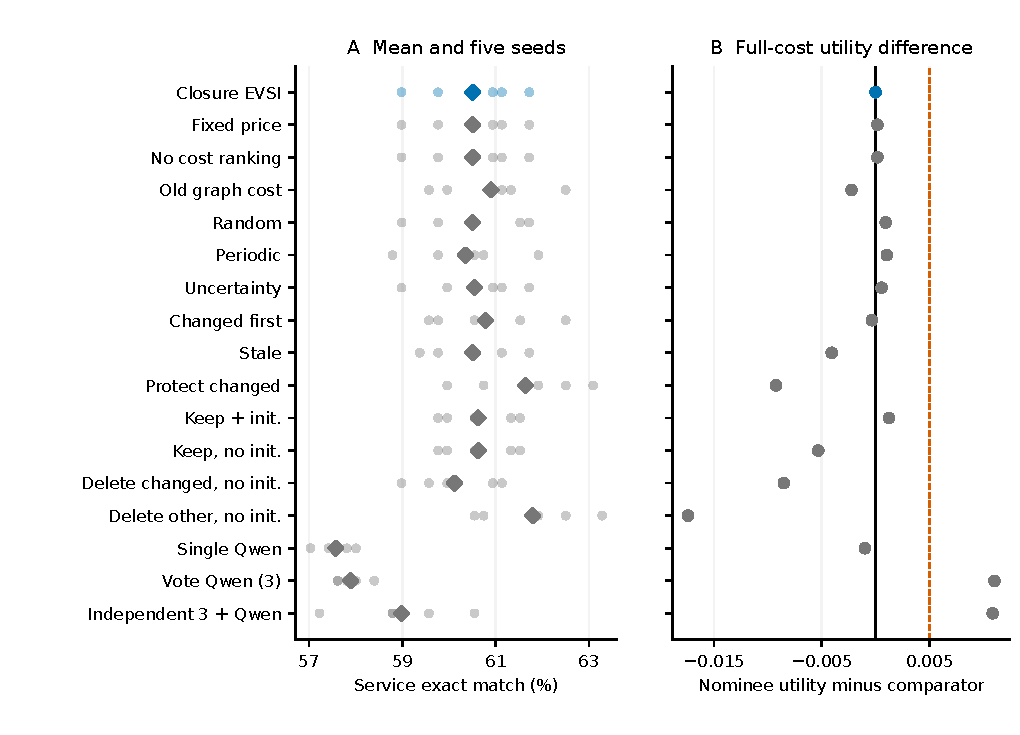
\includegraphics[width=\textwidth]{figures/paper_points.pdf}
\caption{Graph-change point estimates and nominee-minus-comparator utility. Diamonds show mean exact match; small points show all five seeds. The dashed line marks the required $+0.005$ gain for the designated maintenance/free controls; other system gates differ. Complete utility charges initialization, feedback, and service. There are no confidence intervals.}
\label{fig:cost}
\end{figure*}

\section{Discussion and conclusion}
The final experiment tests decision value directly rather than requiring
a new or globally more accurate credit predictor. Nevertheless, removing
the prediction-accuracy requirement does not remove the need for useful
decision information. In this experiment, fewer paid pairs and exact
request reuse do not yield the required utility improvement over random,
stale credit, and free controls.

The negative result is compatible with several mechanisms: sparse gains,
noisy small-sample estimates, insufficient adaptation of old counts,
misspecified marginal outcome models, or a service horizon too short to
amortize feedback. The present comparisons do not uniquely separate these
explanations. Retuning the horizon, weight, or prior using the revealed
service outcomes would create a new exploratory result, not repair the
failed preregistered candidate.

Across the five formal routes, evidence for conditional credit changed
more readily than evidence for beneficial paid maintenance. This suggests
a useful evaluation discipline: compare every acquisition method against
the same predictor, inexpensive structural rules, and a service-quality
baseline, while charging initialization and feedback. Such a discipline
can reject an attractive mechanism claim without rejecting the broader
research question.

The cycle used 76.476912 GPU residence hours of a 160-hour allowance and
exhausted its five-formal-candidate limit. The latter, not the final
candidate failure alone, is the project stopping condition. No sixth
candidate, fresh positive-method confirmation, or second-task validation
was conducted. We release an evidence-bounded negative draft and audit
record, with no claim of submission readiness or general effectiveness.

\section*{Limitations}
This study evaluates a bounded set of hypotheses, not the proposition that
all graph-conditioned credit maintenance is ineffective or effective.
Earlier candidate decisions are retained, including unsuccessful routes.
The current design uses one task, two model checkpoints, a small fixed
graph menu, and a single exogenous topology change per episode. It does not
evaluate long trajectories with repeated graph edits, adversarial drift,
model replacement, or generalization to a second task. A terminal decision
that reverses an initial deletion preference is a restoration proxy, not
an observed delete-and-restore deployment trajectory.
The service graph is selected once per episode after a bounded calibration
window. The periodic baseline schedules feedback within that window; it
is not a continuously interleaved production refresh policy.

All active nodes in the current candidate receive the same full raw
document context. This isolates communication and execution-cost effects
within that access regime; it does not represent agents holding mutually
private evidence. Earlier partial-context experiments are separate cohorts
and cannot establish a causal advantage for the common-context regime.
The model weights may have encountered benchmark material during
pretraining, which our exclusion ledger cannot establish or rule out.

The Dirichlet model is an intentionally simple decision statistic. It
retains old counts and does not infer the true amount of graph-induced
distribution shift. Its marginal edge distributions do not model every
dependence arising from shared questions and baseline executions. The
one-step expected value calculation is not a proof of optimal multi-step
sampling. A graph-topology signal can exist while providing no additional
decision value beyond a static protection rule.

Gold benchmark scoring supplies feedback in replay. Human labeling time,
human financial cost, and production feedback availability were not
measured. Token utility uses a declared research tradeoff, not a monetary
conversion or a common physical price for different model sizes. Kernel
time and GPU residence are separately reported; neither establishes
latency, energy, or monetary savings in an online system. Exact-request
caching reduces data-collection work, while the policy ledger separately
charges the requests each policy would purchase. This is counterfactual
replay, not a live policy deployment.

The common token cap is an upper bound and may be nonbinding. Equal caps
must not be described as equal realized spending. No-initialization static
controls deliberately test whether paying for maintenance is necessary.
Service-prefix curves retain the originally fixed horizon and do not
estimate policies optimized for every shorter horizon.

Repeated generation seeds share question groups and are not additional
independent data samples. We report question support, paired point
differences, correction and breakage counts, and episode and seed
breakdowns. The new experiment uses no confidence intervals or bootstrap;
its frozen numerical gates are resource-allocation criteria, not tests of
statistical significance or population noninferiority. Previous exposed
data and post-hoc analyses cannot supply independent confirmation.

The literature review records whether claims were checked in an abstract
or in specific paper sections. Published graph-optimization systems were
not all independently reimplemented in this study. Comparisons with
internal baselines therefore cannot establish superiority over the full
external state of the art. Computational replays and a separate arithmetic
implementation establish limited verification scope, not independent
human peer review or submission readiness.

\section*{Artifact availability and research accountability}
Code, frozen contracts, aggregate results, and this draft are organized
in the MAB2 research repository. Raw questions, reference answers,
per-question private matrices, weights, and operational credentials are
excluded from the public artifacts. The appendix specifies the reproduction
boundary. AI assistance was used for research execution, coding, evidence
checks, and drafting. Separate arithmetic implementations do not constitute
independent human review. Author identities, affiliations, funding,
conflict-of-interest declarations, and final human approval have not been
provided; they are unresolved rather than inferred. This document has not
been submitted to a venue. Human authors must verify every source and
scientific claim before any submission.

\bibliography{references}
\clearpage
\appendix
\section{Historical diagnostics and unsuccessful routes}
\label{app:history}
These results explain the sequence of research decisions; they are not
additional independent replications of the final candidate. Earlier exposed
evaluation questions remain development data. We retain each original
candidate decision and do not replace a failed nominee with a better-looking
control. The following tables reproduce aggregate point estimates only.

\paragraph{Prediction error did not establish editing value.}
The original G2 experiment used 200 training, 80 tuning and 120 held-out
GSM8K questions, five generation seeds, two anchor graphs and 12 edges.
Its cross-seed squared-risk estimates were 0.001416882 for the edgewise constant
baseline, 0.001541436 for the first-order predictor, and 0.002195856 for the second-order
predictor. Thus the second-order model failed its frozen prediction gate.
These are cross-seed risk estimates, not ordinary empirical MSE values.
Subsequent D2 controls showed that penalizing the intercept can induce
spurious positive edge credit even for a graph-independent constant response.
This is a property of the original objective, not evidence that the original
implementation violated its contract. Removing the intercept penalty reduced
risk, but the fixed D2 nominee achieved 0.000 percentage points of editing
gain on the already exposed evaluation block. It edited 238 of 240 anchors
and therefore did not acquire useful abstention merely by reducing risk.
The D3 graph-only second-order nominee likewise failed its separate
drift-enrichment gate (point estimate -0.001736111).

\paragraph{Mechanism evidence is distinct from system quality.}
The controlled-path experiments C3 and C4 each used a new 96-question
development cohort and two generation seeds. Their topology-sensitive
credit filters passed, yet their frozen graph nominees were worse than
their single-model and independent-aggregation controls (Table~\ref{tab:prior}).
C4 varied receiver identity and access to raw context; the table reports
the preselected full-context Qwen receiver, without selecting a different
factorial cell after outcomes. C3 used a Mistral terminal receiver, whereas
C4's nominated terminal receiver was Qwen. Cohorts and operators differ;
the two rows do not estimate the effect of the receiver change.

\begin{table}[t]
\centering\small
\begin{tabular}{lrrrr}
\hline
Stage & Graph EM & Single Q & Indep. & $D$ \\
\hline
C3 & 35.94 & 51.04 & 57.29 & 0.0625 \\
C4 & 50.52 & 58.85 & 67.71 & 0.1042 \\
\hline
\end{tabular}
\caption{Historical within-cohort comparisons. EM is a percentage;
$D$ is the frozen topology-sensitive credit contrast in its original
proportion units. The independent aggregator is Mistral in C3 and Qwen
in C4. Nonzero question support is 27/96 and 21/96, respectively.
Each row averages two generation seeds on the same question cohort;
seeds are not additional independent question samples.}
\label{tab:prior}
\end{table}

\paragraph{Feedback must beat inexpensive structural controls.}
Post-hoc replay on exposed C3 outputs found that affected-edge refresh
could match a zero-new-feedback protection rule without improving it.
This diagnostic motivated including protection and no-initialization
static actions in the later contract; it does not confirm that contract.
An execution audit also found disconnected source calls in the old operator.
Eliminating those calls is ordinary dead-code elimination and is shared
by every applicable method in the new operator. Accounting savings from
old traces are not measured runtime speedups of the new implementation.

\section{Additional final-candidate results}
Tables~\ref{tab:no_change} and~\ref{tab:weights} retain the complete
no-change comparison and predeclared cost sensitivity. Figure~\ref{fig:prefix}
shows descriptive prefixes of the same fixed policies.
\begin{table*}[t]
\centering\small
\begin{tabular}{lrrrrrr}
\toprule
Method & EM (\%) & F1 (\%) & Utility & Tokens / $S$ item & Pairs & Correct / break \\
\midrule
Closure EVSI (nominee) & 60.430 & 71.646 & 0.560881 & 8683.25 & 6.525 & 62 / 45 \\
EVSI fixed price & 60.430 & 71.646 & 0.560791 & 8701.08 & 6.525 & 62 / 45 \\
EVSI no cost ranking & 60.391 & 71.644 & 0.560400 & 8701.16 & 6.525 & 61 / 45 \\
EVSI old graph cost & 60.430 & 71.646 & 0.560881 & 8683.25 & 6.525 & 62 / 45 \\
Random & 60.508 & 71.732 & 0.561029 & 8809.79 & 8.000 & 64 / 45 \\
Periodic & 60.508 & 71.763 & 0.561496 & 8716.38 & 8.000 & 63 / 44 \\
Uncertainty & 60.469 & 71.685 & 0.560359 & 8865.63 & 8.000 & 62 / 44 \\
Changed first & 60.547 & 71.773 & 0.561855 & 8722.67 & 8.000 & 64 / 44 \\
Stale & 60.430 & 71.646 & 0.563911 & 8077.16 & 0.000 & 64 / 47 \\
Protect changed & 60.430 & 71.646 & 0.563911 & 8077.16 & 0.000 & 64 / 47 \\
Keep (with init.) & 59.766 & 70.968 & 0.556912 & 8148.95 & 0.000 & 0 / 0 \\
Keep (no init.) & 59.766 & 70.968 & 0.563482 & 6834.75 & 0.000 & 0 / 0 \\
Delete changed (no init.) & 60.742 & 71.718 & 0.573606 & 6763.10 & 0.000 & 68 / 43 \\
Delete other (no init.) & 60.312 & 71.543 & 0.569307 & 6763.57 & 0.000 & 61 / 47 \\
Single Qwen & 57.578 & 65.539 & 0.568207 & 1514.93 & 0.000 & 294 / 350 \\
Vote Qwen (3) & 57.891 & 65.895 & 0.556182 & 4544.88 & 0.000 & 300 / 348 \\
Independent 3 + Qwen & 58.984 & 70.520 & 0.556352 & 6698.34 & 0.000 & 191 / 211 \\
\bottomrule
\end{tabular}
\caption{No-change service results. Each method has 512 distinct service questions and 2,560 question--seed observations. Tokens include initialization and feedback; pairs are per episode--seed. Corrections/breakages use the matched keep output. No uncertainty intervals are shown.}
\label{tab:no_change}
\end{table*}

\begin{table*}[t]
\centering\small
\begin{tabular}{lrrrr}
\toprule
Method & $\lambda=0$ & $0.005/1000$ & $0.02/1000$ & $0.05/1000$ \\
\midrule
Closure EVSI (nominee) & 0.605078 & 0.567215 & 0.453627 & 0.226449 \\
EVSI fixed price & 0.605078 & 0.567048 & 0.452957 & 0.224774 \\
EVSI no cost ranking & 0.605078 & 0.567041 & 0.452930 & 0.224708 \\
EVSI old graph cost & 0.608984 & 0.569451 & 0.450852 & 0.213653 \\
Random & 0.605078 & 0.566282 & 0.449894 & 0.217118 \\
Periodic & 0.603516 & 0.566172 & 0.454139 & 0.230074 \\
Uncertainty & 0.605469 & 0.566661 & 0.450237 & 0.217388 \\
Changed first & 0.607812 & 0.567563 & 0.446813 & 0.205314 \\
Stale & 0.605078 & 0.571291 & 0.469928 & 0.267203 \\
Protect changed & 0.616406 & 0.576462 & 0.456630 & 0.216965 \\
Keep (with init.) & 0.606250 & 0.565966 & 0.445116 & 0.203415 \\
Keep (no init.) & 0.606250 & 0.572537 & 0.471400 & 0.269125 \\
Delete changed (no init.) & 0.601172 & 0.575727 & 0.499393 & 0.346725 \\
Delete other (no init.) & 0.617969 & 0.584613 & 0.484547 & 0.284415 \\
Single Qwen & 0.575781 & 0.568207 & 0.545483 & 0.500035 \\
Vote Qwen (3) & 0.578906 & 0.556182 & 0.488009 & 0.351662 \\
Independent 3 + Qwen & 0.589844 & 0.556352 & 0.455877 & 0.254927 \\
\bottomrule
\end{tabular}
\caption{Predeclared descriptive utility sensitivity on the fixed graph-change policies. Policies are not retuned at other weights. The primary weight remains $0.005/1000$.}
\label{tab:weights}
\end{table*}

\begin{figure*}[t]
\centering
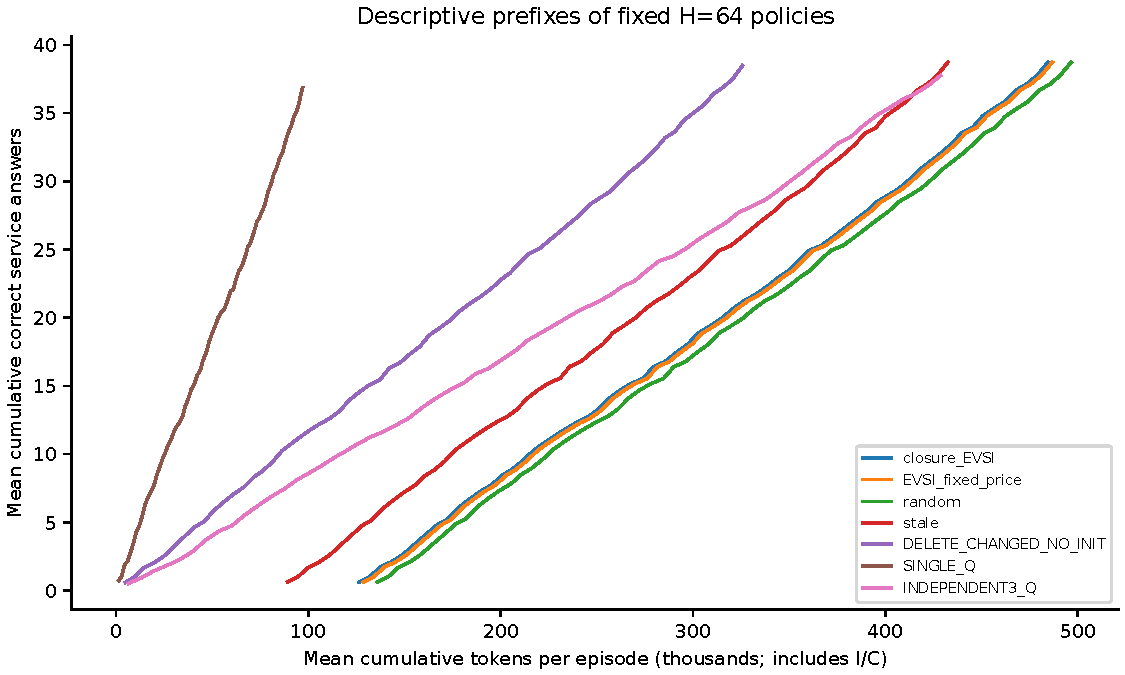
\includegraphics[width=0.95\textwidth]{figures/cumulative_service.pdf}
\caption{Descriptive prefixes of the fixed $H=64$ graph-change policies. The horizontal axis includes all initialization and paid feedback before the first service item; the vertical axis is the mean cumulative number of correct service answers per episode--seed. Policies are not retrained or reoptimized at each prefix. These curves do not establish an optimized equal-spend frontier.}
\label{fig:prefix}
\end{figure*}

\section{Reproduction boundary}
The public aggregate generator reconstructs both 17-method tables,
all five nominee seed points, and the four-weight sensitivity table from
the frozen summary. It reconciles 1,360 episode--seed rows against totals.
The historical generator binds its tables to seven historical source
files by SHA-256. No generator fits a model or resamples data.

The portable experiment bundle passes 36 artificial tests. With authorized
access to private archives, the request auditor reconstructs prompts,
seeds, cache decisions, and stored outputs without model calls. The
independent raw scorer recomputes normalization, exact match, token F1,
and all 3,200 voting decisions; the independent policy auditor rebuilds
paid ledgers and fixed gates. These checks verify limited implementation
properties. They do not regenerate stochastic outputs, supply a new
evaluation cohort, or constitute human review.

The public cost ledger has 11 closed entries: five formal candidates and
six separate engineering qualifications. Cycle GPU residence sums across
workers, including loading and waiting. Historical G2 CUDA-event time
is a separate measurement and is not added to residence or recharged to
this cycle. Unknown human, financial, energy, and complete agent-execution
costs are not imputed as zero. Per-policy logical charges must not be
summed across mutually exclusive policies and interpreted as actual
collection expenditure.

The released code and aggregate artifacts support computational inspection
without exposing raw question-level records. Full private replay requires
the corresponding owner-controlled archive, selection record, approval
files, and pinned model/tokenizer environment. This privacy boundary limits
what an unaffiliated reader can reproduce from public Git alone.

\end{document}
